% !TEX root=../root.tex

\subsection{Experiment Results}
% The multirotor UAV was manually flown until the
% fiducial landing marker was detected. Upon detection, the closed-loop estimation
% and control system took full control of the UAV.

The results of the flight experiment are shown in~\figref{fig:est_hardware}.
The fiducial landing marker was first detected at $t = 20$ s, where the plots
begin.
To demonstrate the ability of the
system to maintain good tracking of a target vehicle when a fiducial
marker is not detected for long periods of time, the fiducial marker detection
was turned off ten seconds after initial detection, at $t = 30$ s.
% The fiducial landing marker was first detected at
% $t = 20$ s and last detected at $t = 30$ s.
It is clear that the estimates of the position, velocity, attitude, and angular
velocity of the target vehicle remained accurate and consistent for the duration
of the experiment.
% despite no measurements from the fiducial marker being used
% after $t = 30$ s.
% Even though no measurements from the fiducial marker are used, it is clear that
% the estimates of the position, velocitity, attitude and angular velocity of the
% target vehicle remain accurate and consistent for the duration of the
% experiment.
These accurate estimates allowed
the UAV to continue to control relative to the target vehicle, tracking closely
above the landing target as the target vehicle moved around the room. After the
target vehicle completed two full laps around the room,
at approximately $t=102$ s, manual control of the UAV was resumed, ending the experiment.
A video of the flight experiment can be found at
\url{https://youtu.be/3AyjCI0c1Nc}.
% \url{https://youtu.be/VU5sq6FuSL0}.

\begin{figure}
  \centering
  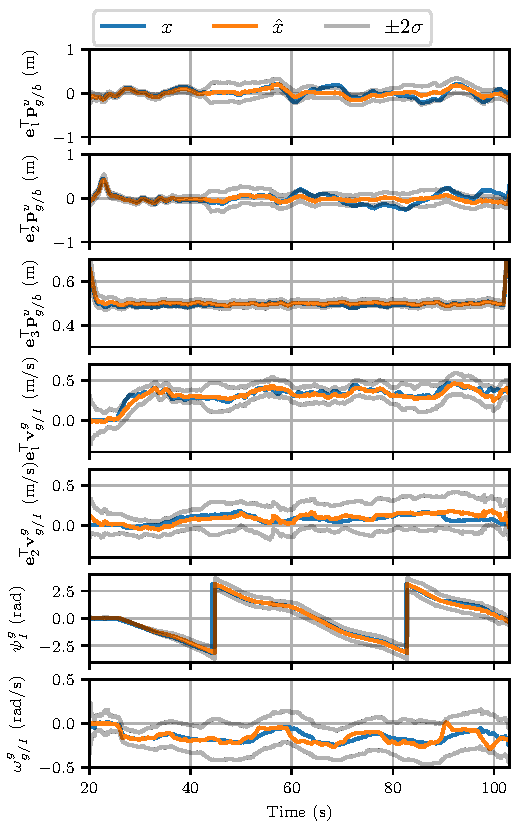
\includegraphics[width=6.5in]{plots/hardware_results}
  \caption[ESKF Hardware Results Using Ten Visual Features]{Hardware results when
    the ESKF estimated the positions of \emph{ten} visual
  features. The blue line represents the true state while the orange line
  represents the estimated state. The two grey lines show $\pm 2 \sigma$ bounds for
  the estimate based on the estimated covariance. Measurements from the fiducial
  marker were not used after $t = 30$ s to demonstrate the performance of the estimator.}
  \label{fig:est_hardware}
\end{figure}
